\chapter{The First G-APD Cherenkov Telescope}\label{chp:fact}
\begin{figure}
  \centering
  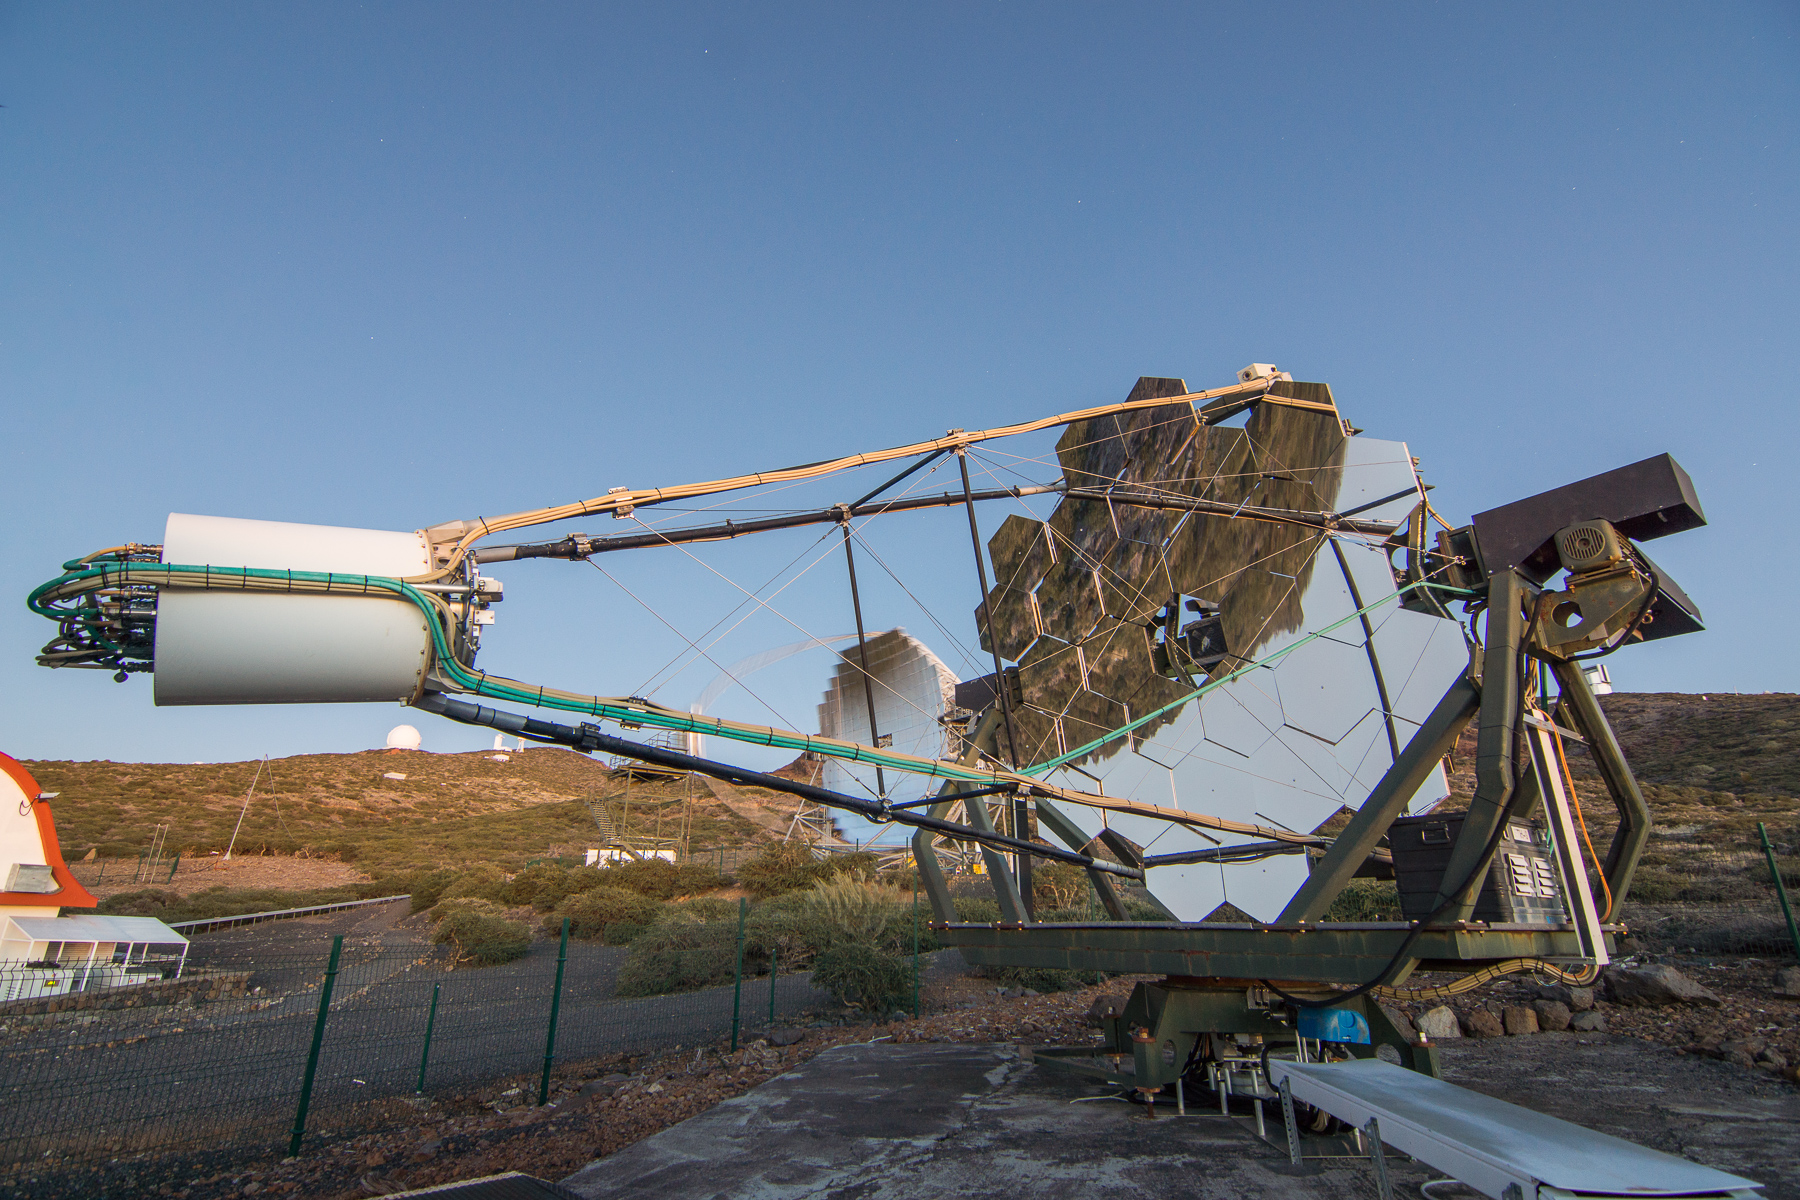
\includegraphics[width=\textwidth]{images/fact.jpg}
  \caption{%
    \gls{fact} in front of the \gls{magic}-II telescope at the Observatorio del Roque de los Muchachos.
    The white cylinder on the left is the camera, complete with all readout electronics.
    }%
  \label{fig:a}
\end{figure}


\noindent In this chapter, I will introduce the necessary aspects
of the \gls{fact} telescope, which are needed to understand the simulation
and analysis presented in the next chapters.

After a general introduction,
I will focus mainly on the data acquisition and electronics,
as these are the parts of the telescope that are most crucial for my work
on improving preprocessing of raw data and simulations.

\begin{wrapfigure}[25]{O}{0.55\textwidth}
  \centering
  \includegraphics{build/plots/fact_ontime_half.pdf}
  \caption{%
    Observation time for the seven sources most observed by \gls{fact}. 
    Together they amount to over \SI{95}{\percent} of the total time the telescope
    has observed.
  }\label{fig:obstime}
\end{wrapfigure}

One of the main goals of \gls{fact} was to demonstrate the possibility
of using \glspl{sipm} for Cherenkov astronomy~\cite{fact-design-operation}.
It has been the first telescope to employ this new technology of photodetectors
in the field when it started operating in 2011.
Now, eight years later, all prototypes for the \gls{sst} for \gls{cta} are based 
on \gls{sipm} cameras and the final design was agreed upon in 2019~
\cite{sst-harmonization}. 
It can be safely concluded that \gls{fact} reached this goal.

Compared to the traditionally used \glspl{pmt},
these semiconductor photosensors are much more robust to high light levels.
Due to this, \gls{fact} can observe under light conditions,
e.\,g.\ in moonlit nights, where other \glspl{iact} can not~\cite{fact_full_moon}.
This makes \gls{fact} uniquely suited for its main physics goal,
to monitor the brightest sources of gamma rays as densely as possible,
which is also evident in \autoref{fig:obstime},
showing that \gls{fact} spends most of its observation time on just seven sources.
Shortly after starting observations in October 2011,
the \gls{fact} collaboration started publishing
results of a \enquote{quick look analysis}~\cite{qla} as soon as they were available.
This analysis provides gamma-ray event rates normally around 20 minutes after the last event of a run was taken.
Based on this analysis, the \gls{fact} collaboration has issued
several alerts to the other \glspl{iact} to inform them of unusually bright
flux of the monitored sources~\cite{fact_alerts}.

\gls{fact} is build upon the refurbished mount of the former \gls{hegra} CT-3 telescope,
equipped with new drive motors, mirrors and the \gls{sipm} camera.
Compared to the other currently operating telescopes, like \gls{veritas} or \gls{magic},
\gls{fact} is rather small, limiting its sensitivity to the brightest sources.
It is also the only currently operating monoscopic Cherenkov observatory.
\gls{fact}'s reflector is a segmented mirror with 30 individual hexagonal facets,
creating a total reflective surface of \SI{9.5}{\square\meter} with approximately four
meters in diameter.
Each mirror as a focal length of \SI{4.9}{\meter}, which is also the effective focal 
length of the segmented reflector.
The facets were oriented in the Davies--Cotton-Design\cite{davies-cotton} before this
was changed to a hybrid between Davies--Cotton and a parabolic orientation
in May 2014, as a compromise between spatial and temporal resolution of the reflector system~\cite{mirror-alignment}.
At this point, the mirrors were also realigned, resulting in an overall better resolution
than before.

\section{Photosensors and Readout Electronics}\label{sec:camera}

\gls{fact}'s camera comprises 1440 pixels,
each consisting of a \SI{3}{\milli\meter} by \SI{3}{\milli\meter} \gls{sipm}
that is subdivided into 3600 individual \gls{gapd} cells.
\glspl{gapd} are photodiodes operated with a reverse bias above the breakdown voltage,
the limit above which a single electron/hole pair created by an absorbed photon can induce an avalanche.
The cell is connected in series to a resistor and the current created
by the avalanche results in dropping the bias below the breakdown breakdown, 
stopping the avalanche.
After an avalanche, the cell needs a short time to reset to the full bias voltage again.
During the dead time, while the cell is below the breakdown voltage,
no new signal can be created.
While it is above the breakdown but below the nominal operation voltage—called recovery time—,
the signal is lower than normally~\cite{fact-design-operation}.
The single cells are connected in parallel to form a single, accumulated output signal
per pixel.
\glspl{sipm} do not need a high voltage supply in the \si{\kilo\volt} regime like \glspl{pmt} do.
\gls{fact}'s photosensors have a breakdown voltage around \SI{70}{\volt} and
are operated at an overvoltage of \SI{1}{\volt}, 
while some more recent models even only require \SI{30}{\volt}~\cite{sensl}.

However, \glspl{sipm} do not come without issues.
One disadvantage is the temperature dependent gain of \glspl{sipm} and two
main approaches exist to deal with this: active cooling of the sensors to a
fixed temperature or a system adjusting the bias voltage of the \glspl{sipm} 
so the gain stays stable.
\gls{fact} has implemented the second path, only relying on removing excess heat
from the camera, not keeping a fixed temperature for observations.
The bias voltage is generated in the container next to the telescope and supplied
to groups of 4 or 5 pixels, called bias patches shown in \autoref{fig:pixels}.~\cite{fact-design-operation}

Compared to \glspl{pmt} they have a higher dark count rate,
signals induced not by photons but by thermal electrons in the sensor itself.
Cross talk, the effect that a break through in one cell can trigger another in a neighboring cell,
results in a signal corresponding to two photons or more.
There is also a chance  that a discharge triggers a later discharge of the same cell,
which is called an after pulse.~\cite{cross-talk}

To increase the light gathering surface area, a Winston cone with a hexagonal
entry window with an incircle diameter of \SI{9.5}{\milli\meter} is placed in front of each pixel.
The resulting camera is roughly \SI{40}{\centi\meter} in diameter which, together with
the \SI{4.9}{\meter} focal length of the reflector, gives a field of view of \SI{4.5}{\degree}.
Each individual pixel covers \SI{0.11}{\degree} in diameter on the sky.

\begin{figure}
  \begin{captionbeside}{
    Schematic view of the camera. From left to right: the 1440 pixels in the 
    sensor compartment, the insulation between sensor compartment and
    readout electronics, the 4 crates with the preamplifier boards and the 
    \gls{fadc} boards. The \gls{ftm} can be seen at the top next to the insulation.\\\relax
    [Graphic by Sebastian~A.~Mueller]
  }
    \raisebox{\dimexpr\baselineskip-\totalheight\relax}{%
      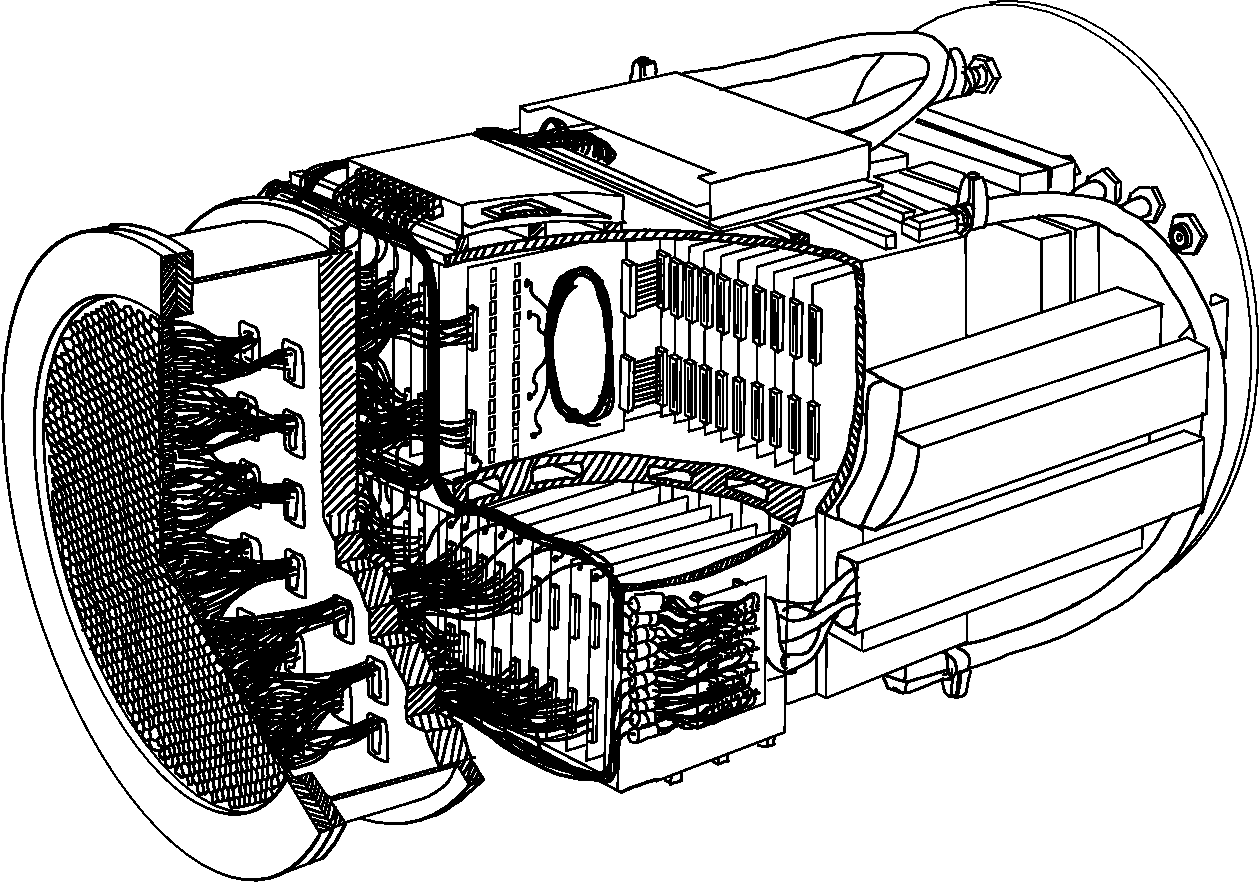
\includegraphics[width=0.6\linewidth]{images/image_sensor.pdf}
    }% 
  \end{captionbeside}\label{fig:camera}
\end{figure}

The analog signal of the pixels is wired to the preamplifier boards, that handle
36 pixels each and are organized in four crates of ten boards of the preamplifier
and \gls{fadc} boards each.
The trigger unit on the preamplifier board clips and sums the signal of 9 pixels each,
these groups are referred to as trigger patches. 
The preamplifier board applies an $N$-out-of-four logic to these trigger input signals,
which is the input for the \gls{ftm} board, which applies a $N$-out-of-40 logic to
decide if an event should be stored to disk.
For normal physics observations, both $N$ are 1, thus if any of the 160 trigger patches
is above the trigger threshold, an event is stored to disk.
In addition to events triggered by this system, additional events are recorded
during normal data runs.
The camera is read out once per second regardless of a trigger signal, these
are so called interleaved pedestal events which can be used to estimate the noise
level.
Since November 2013, the camera is also triggered at every full second by a GPS
receiver to provide more precise timing information.
Until 2017, an LED light pulser in the reflector dish fired every few seconds,
this was done for calibration of the pixel response.
However, this LED light pulser went rogue in 2015 and also fired without being activated
creating large events triggered by the physics trigger until it was finally removed in April 2016.

The \gls{fadc} boards also receive their signal from the preamplifier boards.
The heart of the \glspl{fadc} are the \gls{drs4} chips~\cite{drs4}. 
These chips sample the analog signal using 1024 capacitors for each channel using
a sampling frequency of \SI{2}{\giga Sample \per \second}.
In case the \gls{ftm} issues a trigger decision, the voltage stored in the capacitors
is readout and digitized by a 12-bit \gls{adc}.
For regular observations, only 300 of the samples are readout, starting 50 samples
before the trigger signal was received \cite{fact-design-operation}.
While the \gls{drs4} chips allow fast digitization of the \gls{sipm} signal,
it also introduces the need for several calibration steps
and adds artifacts to the data~\cite{magic-drs4}.
The most common artifacts are sudden increases of the digitized signal in a single
or two adjacent cells called spikes.
These interfere with the searching for the Cherenkov pulse signal if not corrected.
Different amounts of remaining charge in the cells are responsible for sudden shifts of the baseline
for longer time periods when reading out cells that have had different times since their previous readout.
In \gls{fact}'s terminology, these are called jumps.

The digitized samples are transferred via four ethernet connections to the data acquisition computer which writes the data to disk. 
Under good environmental conditions \gls{fact} triggers between 60 and 80 events per seconds
\cite{fact-sipm-performance,fact-design-operation}.
The organization of the \gls{fact} camera pixels into the different groups is shown in
\autoref{fig:pixels}.

\begin{figure}
  \centering
  \includegraphics{build/plots/fact_pixels.pdf}
  \caption{%
    Organization of the \gls{fact} camera.
    The four main colors highlight the crates, the variation in those colors the 
    boards.
    The left image shows the individual pixels.
    In the central image, pixels using the same bias voltage supply are grouped.
    The right image shows all pixels on the same \gls{drs4} chip, which also corresponds
    to the trigger patches.
  }\label{fig:pixels}
\end{figure}

\section{Observation Strategy}\label{sec:wobble}

As not all recorded background events can be discarded reliably while still
keeping most of the gamma rays, a method to estimate this residual background is needed.
A simple method would be to observe the gamma-ray source first and then 
observe a similar region in the sky without a gamma-ray source for the background estimation.
This has several important drawbacks,
first the available time for source observations is cut in half.
Second, the observation conditions might change and thus bias the estimation of the background.

A way around this is not to position the source of interest in the center of the 
camera but using a small offset.
In this case, several regions in the camera geometrically
equivalent to the position of the gamma-ray source can be used for the background estimation.
This maximizes observation time for gamma-ray sources, guarantees identical observation
conditions for the background estimation and also decreases the
statistical uncertainty for the background, as several positions can be used~\cite{wobble}.
The situation is sketched in \autoref{fig:wobble}.
Nearly all \gls{fact} observations are carried out in this manner.
Due do the characteristic switching between positions relative to the source,
making small jumps around its position, this strategy is called \enquote{wobble mode}.

\begin{figure}
  \centering
  \begin{tikzpicture}
  \newlength\mydeg
  \setlength{\mydeg}{2cm}

  \pgfdeclarelayer{bg}
  \pgfsetlayers{bg,main}

  
  \node[star, star points=5, fill=yellow!80!red, minimum height=0.3cm] (source)  at (0, 0) {};

  \node[draw=darkBlue, cross out, line width=2pt, minimum height=0.3cm] (p1) at (-0.6\mydeg, 0) {};
  \node[draw=darkRed, cross out, line width=2pt, minimum height=0.3cm] (p2) at (0.6\mydeg, 0) {};

  \begin{pgfonlayer}{bg}
    \draw[thick, black!20, dashed] (p2) circle (0.6\mydeg);
    \draw[thick, black!20, dashed] (p1) circle (0.6\mydeg);
  \end{pgfonlayer}

  \draw[thick, darkBlue] (p1) circle (2.25\mydeg);
  \draw[thick, darkRed] (p2) circle (2.25\mydeg);

  \foreach \ang in {60,120,180,240,300} {
    \path (p1) -- ++ (\ang:0.6\mydeg) node[circle, minimum height=0.3cm, fill=blue!50!black] {};
  }
  \foreach \ang in {0,60,120,240,300} {
    \path (p2) -- ++ (\ang:0.6\mydeg) node[circle, minimum height=0.3cm, fill=red!50!black] {};
  }

  \draw[{Bar[]Triangle[]}-{Triangle[]Bar[]}] ([yshift=-0.3cm]p1.center) -- ([yshift=-0.3cm]source.center) node [midway, above] {\SI{0.6}{\degree}};
\end{tikzpicture}

  \caption{%
    When observing a source in wobble mode, the source (yellow star) is not in the center (crosses) of the field of view but offset by a certain amount.
    \gls{fact} uses \SI{0.6}{\degree}. 
    Shown here are two wobble positions at wobble angles of \SI{0}{\degree} (red) and \SI{180}{\degree} (blue) as measured from the right ascension axis.
    \gls{fact} normally observes using two wobble positions at \SI{180}{\degree} offsets,
    changing position every twenty minutes.
    The bold circles show the five off positions per pointing position that are
    used to estimate the background.
    Because there is a bright star in the field of view for Crab Nebula observations,
    the wobble angles are shifted by \SI{50}{\degree}, so the star is not close to
    any of the off positions.
  }\label{fig:wobble}
\end{figure}
